% Options for packages loaded elsewhere
\PassOptionsToPackage{unicode}{hyperref}
\PassOptionsToPackage{hyphens}{url}
%
\documentclass[
]{article}
\usepackage{amsmath,amssymb}
\usepackage{iftex}
\ifPDFTeX
  \usepackage[T1]{fontenc}
  \usepackage[utf8]{inputenc}
  \usepackage{textcomp} % provide euro and other symbols
\else % if luatex or xetex
  \usepackage{unicode-math} % this also loads fontspec
  \defaultfontfeatures{Scale=MatchLowercase}
  \defaultfontfeatures[\rmfamily]{Ligatures=TeX,Scale=1}
\fi
\usepackage{lmodern}
\ifPDFTeX\else
  % xetex/luatex font selection
\fi
% Use upquote if available, for straight quotes in verbatim environments
\IfFileExists{upquote.sty}{\usepackage{upquote}}{}
\IfFileExists{microtype.sty}{% use microtype if available
  \usepackage[]{microtype}
  \UseMicrotypeSet[protrusion]{basicmath} % disable protrusion for tt fonts
}{}
\makeatletter
\@ifundefined{KOMAClassName}{% if non-KOMA class
  \IfFileExists{parskip.sty}{%
    \usepackage{parskip}
  }{% else
    \setlength{\parindent}{0pt}
    \setlength{\parskip}{6pt plus 2pt minus 1pt}}
}{% if KOMA class
  \KOMAoptions{parskip=half}}
\makeatother
\usepackage{xcolor}
\usepackage[margin=1in]{geometry}
\usepackage{color}
\usepackage{fancyvrb}
\newcommand{\VerbBar}{|}
\newcommand{\VERB}{\Verb[commandchars=\\\{\}]}
\DefineVerbatimEnvironment{Highlighting}{Verbatim}{commandchars=\\\{\}}
% Add ',fontsize=\small' for more characters per line
\usepackage{framed}
\definecolor{shadecolor}{RGB}{248,248,248}
\newenvironment{Shaded}{\begin{snugshade}}{\end{snugshade}}
\newcommand{\AlertTok}[1]{\textcolor[rgb]{0.94,0.16,0.16}{#1}}
\newcommand{\AnnotationTok}[1]{\textcolor[rgb]{0.56,0.35,0.01}{\textbf{\textit{#1}}}}
\newcommand{\AttributeTok}[1]{\textcolor[rgb]{0.13,0.29,0.53}{#1}}
\newcommand{\BaseNTok}[1]{\textcolor[rgb]{0.00,0.00,0.81}{#1}}
\newcommand{\BuiltInTok}[1]{#1}
\newcommand{\CharTok}[1]{\textcolor[rgb]{0.31,0.60,0.02}{#1}}
\newcommand{\CommentTok}[1]{\textcolor[rgb]{0.56,0.35,0.01}{\textit{#1}}}
\newcommand{\CommentVarTok}[1]{\textcolor[rgb]{0.56,0.35,0.01}{\textbf{\textit{#1}}}}
\newcommand{\ConstantTok}[1]{\textcolor[rgb]{0.56,0.35,0.01}{#1}}
\newcommand{\ControlFlowTok}[1]{\textcolor[rgb]{0.13,0.29,0.53}{\textbf{#1}}}
\newcommand{\DataTypeTok}[1]{\textcolor[rgb]{0.13,0.29,0.53}{#1}}
\newcommand{\DecValTok}[1]{\textcolor[rgb]{0.00,0.00,0.81}{#1}}
\newcommand{\DocumentationTok}[1]{\textcolor[rgb]{0.56,0.35,0.01}{\textbf{\textit{#1}}}}
\newcommand{\ErrorTok}[1]{\textcolor[rgb]{0.64,0.00,0.00}{\textbf{#1}}}
\newcommand{\ExtensionTok}[1]{#1}
\newcommand{\FloatTok}[1]{\textcolor[rgb]{0.00,0.00,0.81}{#1}}
\newcommand{\FunctionTok}[1]{\textcolor[rgb]{0.13,0.29,0.53}{\textbf{#1}}}
\newcommand{\ImportTok}[1]{#1}
\newcommand{\InformationTok}[1]{\textcolor[rgb]{0.56,0.35,0.01}{\textbf{\textit{#1}}}}
\newcommand{\KeywordTok}[1]{\textcolor[rgb]{0.13,0.29,0.53}{\textbf{#1}}}
\newcommand{\NormalTok}[1]{#1}
\newcommand{\OperatorTok}[1]{\textcolor[rgb]{0.81,0.36,0.00}{\textbf{#1}}}
\newcommand{\OtherTok}[1]{\textcolor[rgb]{0.56,0.35,0.01}{#1}}
\newcommand{\PreprocessorTok}[1]{\textcolor[rgb]{0.56,0.35,0.01}{\textit{#1}}}
\newcommand{\RegionMarkerTok}[1]{#1}
\newcommand{\SpecialCharTok}[1]{\textcolor[rgb]{0.81,0.36,0.00}{\textbf{#1}}}
\newcommand{\SpecialStringTok}[1]{\textcolor[rgb]{0.31,0.60,0.02}{#1}}
\newcommand{\StringTok}[1]{\textcolor[rgb]{0.31,0.60,0.02}{#1}}
\newcommand{\VariableTok}[1]{\textcolor[rgb]{0.00,0.00,0.00}{#1}}
\newcommand{\VerbatimStringTok}[1]{\textcolor[rgb]{0.31,0.60,0.02}{#1}}
\newcommand{\WarningTok}[1]{\textcolor[rgb]{0.56,0.35,0.01}{\textbf{\textit{#1}}}}
\usepackage{graphicx}
\makeatletter
\def\maxwidth{\ifdim\Gin@nat@width>\linewidth\linewidth\else\Gin@nat@width\fi}
\def\maxheight{\ifdim\Gin@nat@height>\textheight\textheight\else\Gin@nat@height\fi}
\makeatother
% Scale images if necessary, so that they will not overflow the page
% margins by default, and it is still possible to overwrite the defaults
% using explicit options in \includegraphics[width, height, ...]{}
\setkeys{Gin}{width=\maxwidth,height=\maxheight,keepaspectratio}
% Set default figure placement to htbp
\makeatletter
\def\fps@figure{htbp}
\makeatother
\setlength{\emergencystretch}{3em} % prevent overfull lines
\providecommand{\tightlist}{%
  \setlength{\itemsep}{0pt}\setlength{\parskip}{0pt}}
\setcounter{secnumdepth}{-\maxdimen} % remove section numbering
\ifLuaTeX
  \usepackage{selnolig}  % disable illegal ligatures
\fi
\usepackage{bookmark}
\IfFileExists{xurl.sty}{\usepackage{xurl}}{} % add URL line breaks if available
\urlstyle{same}
\hypersetup{
  pdftitle={R Notebook},
  hidelinks,
  pdfcreator={LaTeX via pandoc}}

\title{R Notebook}
\author{}
\date{\vspace{-2.5em}}

\begin{document}
\maketitle

{
\setcounter{tocdepth}{2}
\tableofcontents
}
Load the libraries

Set the factors

\begin{Shaded}
\begin{Highlighting}[]
\NormalTok{treatment\_pattern }\OtherTok{\textless{}{-}}\NormalTok{ (}\FunctionTok{rep}\NormalTok{(}\FunctionTok{c}\NormalTok{(}\StringTok{"Untreated"}\NormalTok{, }\StringTok{"Treatment"}\NormalTok{), }\AttributeTok{times =} \DecValTok{9}\NormalTok{))}
\NormalTok{treatment }\OtherTok{\textless{}{-}} \FunctionTok{factor}\NormalTok{(}\FunctionTok{c}\NormalTok{(treatment\_pattern))}

\NormalTok{donor\_pattern }\OtherTok{\textless{}{-}} \FunctionTok{c}\NormalTok{(}\FunctionTok{rep}\NormalTok{(}\StringTok{"M24"}\NormalTok{, }\AttributeTok{times =} \DecValTok{6}\NormalTok{), }\FunctionTok{rep}\NormalTok{(}\StringTok{"M31"}\NormalTok{, }\AttributeTok{times =} \DecValTok{6}\NormalTok{), }\FunctionTok{rep}\NormalTok{(}\StringTok{"M32"}\NormalTok{, }\AttributeTok{times =} \DecValTok{6}\NormalTok{))}
\NormalTok{donors }\OtherTok{\textless{}{-}} \FunctionTok{factor}\NormalTok{(}\FunctionTok{c}\NormalTok{(donor\_pattern))}
\end{Highlighting}
\end{Shaded}

Cbind the factors

\begin{Shaded}
\begin{Highlighting}[]
\NormalTok{groups }\OtherTok{\textless{}{-}} \FunctionTok{data.frame}\NormalTok{(}\AttributeTok{sample =} \FunctionTok{colnames}\NormalTok{(counts), treatment, donors)}

\FunctionTok{cbind}\NormalTok{(groups,}\FunctionTok{colnames}\NormalTok{(counts))}
\end{Highlighting}
\end{Shaded}

\begin{verbatim}
##          sample treatment donors colnames(counts)
## 1    CF_M24_EV1 Untreated    M24       CF_M24_EV1
## 2  CF_M24_EVPA1 Treatment    M24     CF_M24_EVPA1
## 3    CF_M24_EV2 Untreated    M24       CF_M24_EV2
## 4  CF_M24_EVPA2 Treatment    M24     CF_M24_EVPA2
## 5    CF_M24_EV3 Untreated    M24       CF_M24_EV3
## 6  CF_M24_EVPA3 Treatment    M24     CF_M24_EVPA3
## 7    CF_M31_EV1 Untreated    M31       CF_M31_EV1
## 8  CF_M31_EVPA1 Treatment    M31     CF_M31_EVPA1
## 9    CF_M31_EV2 Untreated    M31       CF_M31_EV2
## 10 CF_M31_EVPA2 Treatment    M31     CF_M31_EVPA2
## 11   CF_M31_EV3 Untreated    M31       CF_M31_EV3
## 12 CF_M31_EVPA3 Treatment    M31     CF_M31_EVPA3
## 13   CF_M32_EV1 Untreated    M32       CF_M32_EV1
## 14 CF_M32_EVPA1 Treatment    M32     CF_M32_EVPA1
## 15   CF_M32_EV2 Untreated    M32       CF_M32_EV2
## 16 CF_M32_EVPA2 Treatment    M32     CF_M32_EVPA2
## 17   CF_M32_EV3 Untreated    M32       CF_M32_EV3
## 18 CF_M32_EVPA3 Treatment    M32     CF_M32_EVPA3
\end{verbatim}

\#\#Part 1 -- Exploratory Analysis\#\# \#\#\#1. Visualize your library
sizes.\#\#\#

\begin{Shaded}
\begin{Highlighting}[]
\FunctionTok{boxplot}\NormalTok{(}\FunctionTok{colSums}\NormalTok{(counts) }\SpecialCharTok{\textasciitilde{}}\NormalTok{ donors)}
\end{Highlighting}
\end{Shaded}

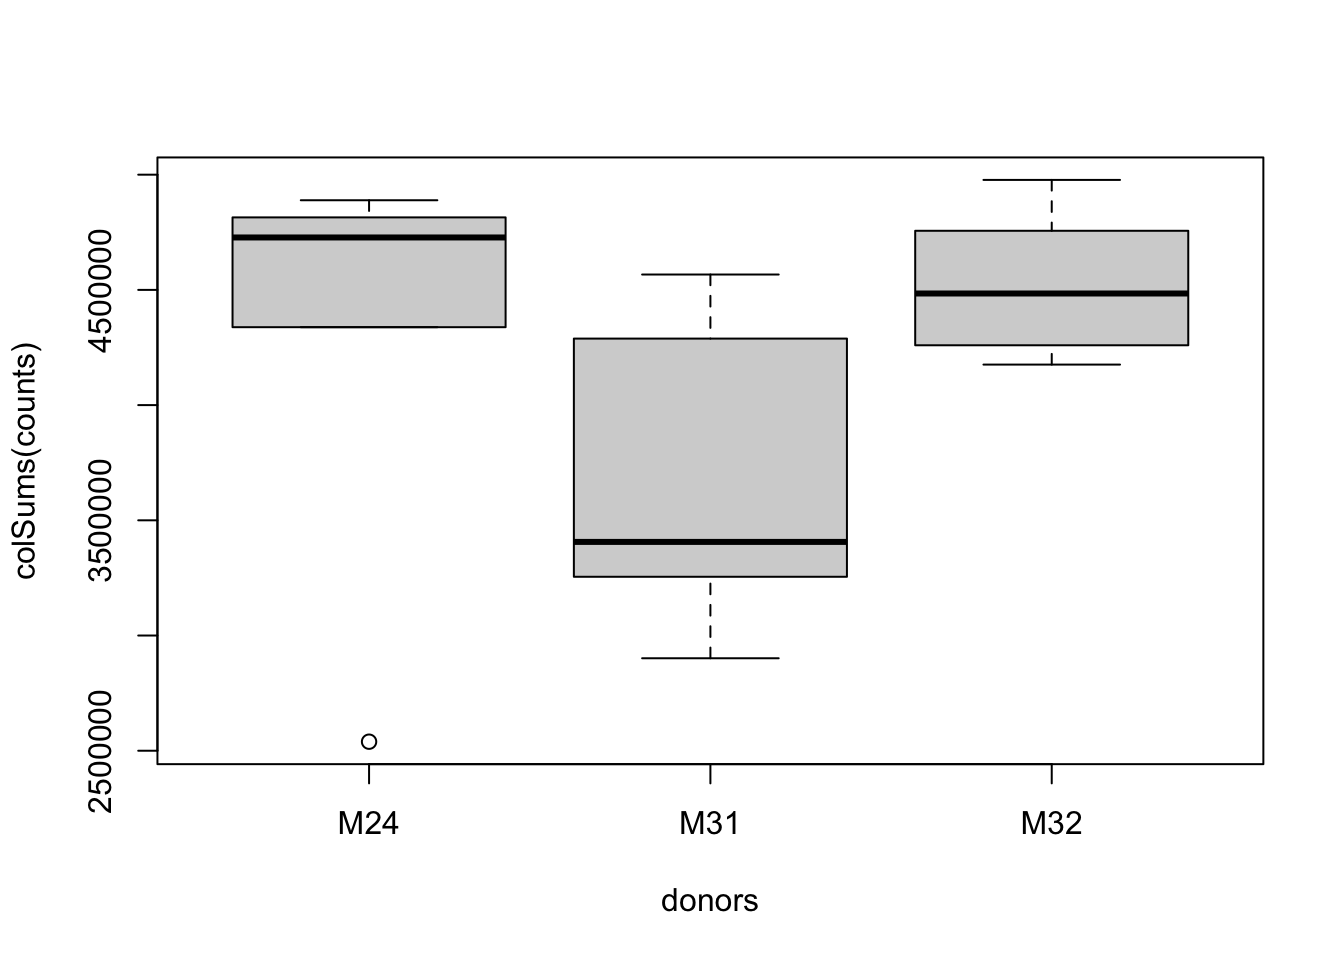
\includegraphics{Clean_files/figure-latex/unnamed-chunk-4-1.pdf}

\begin{Shaded}
\begin{Highlighting}[]
\FunctionTok{boxplot}\NormalTok{(}\FunctionTok{colSums}\NormalTok{(counts) }\SpecialCharTok{\textasciitilde{}}\NormalTok{ treatment)}
\end{Highlighting}
\end{Shaded}

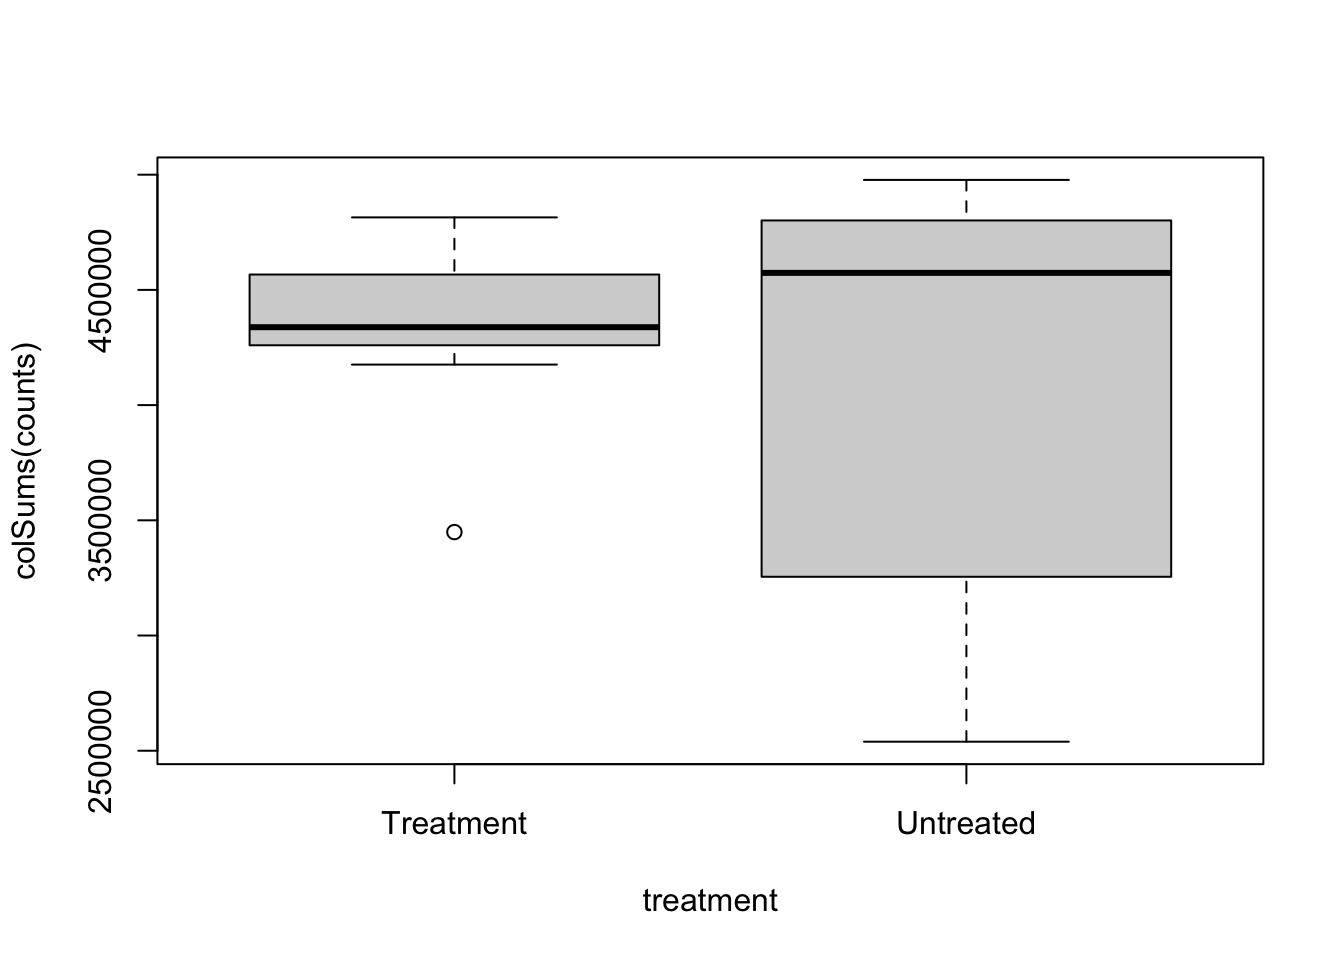
\includegraphics{Clean_files/figure-latex/unnamed-chunk-5-1.pdf}

\begin{Shaded}
\begin{Highlighting}[]
\FunctionTok{boxplot}\NormalTok{(}\FunctionTok{colSums}\NormalTok{(counts) }\SpecialCharTok{\textasciitilde{}}\NormalTok{ groups}\SpecialCharTok{$}\NormalTok{sample)}
\end{Highlighting}
\end{Shaded}

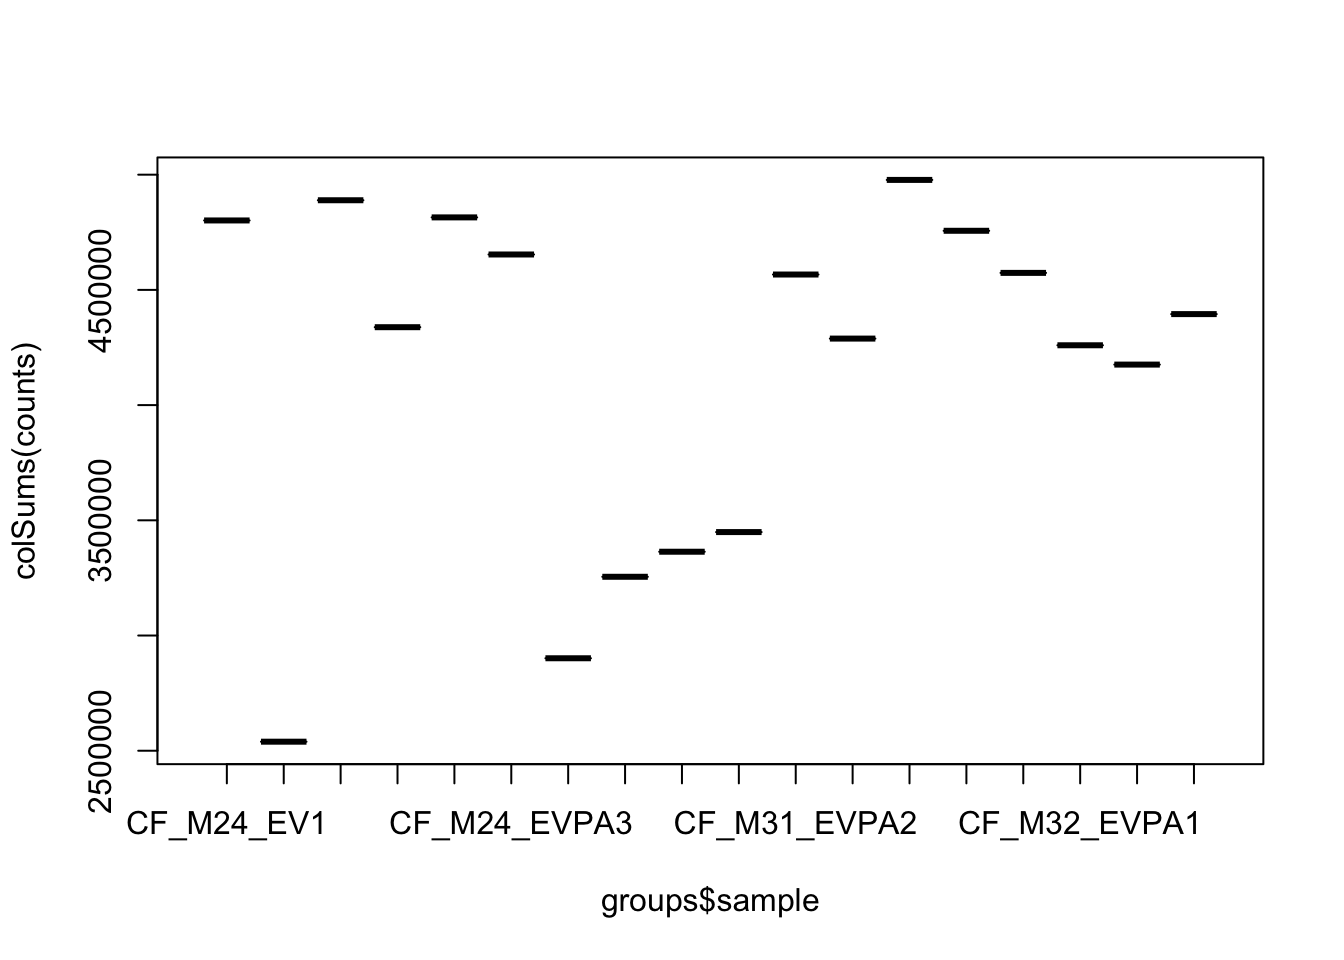
\includegraphics{Clean_files/figure-latex/unnamed-chunk-6-1.pdf}

\begin{Shaded}
\begin{Highlighting}[]
\FunctionTok{hist}\NormalTok{(}\FunctionTok{log2}\NormalTok{(}\FunctionTok{rowSums}\NormalTok{(counts)))}
\end{Highlighting}
\end{Shaded}

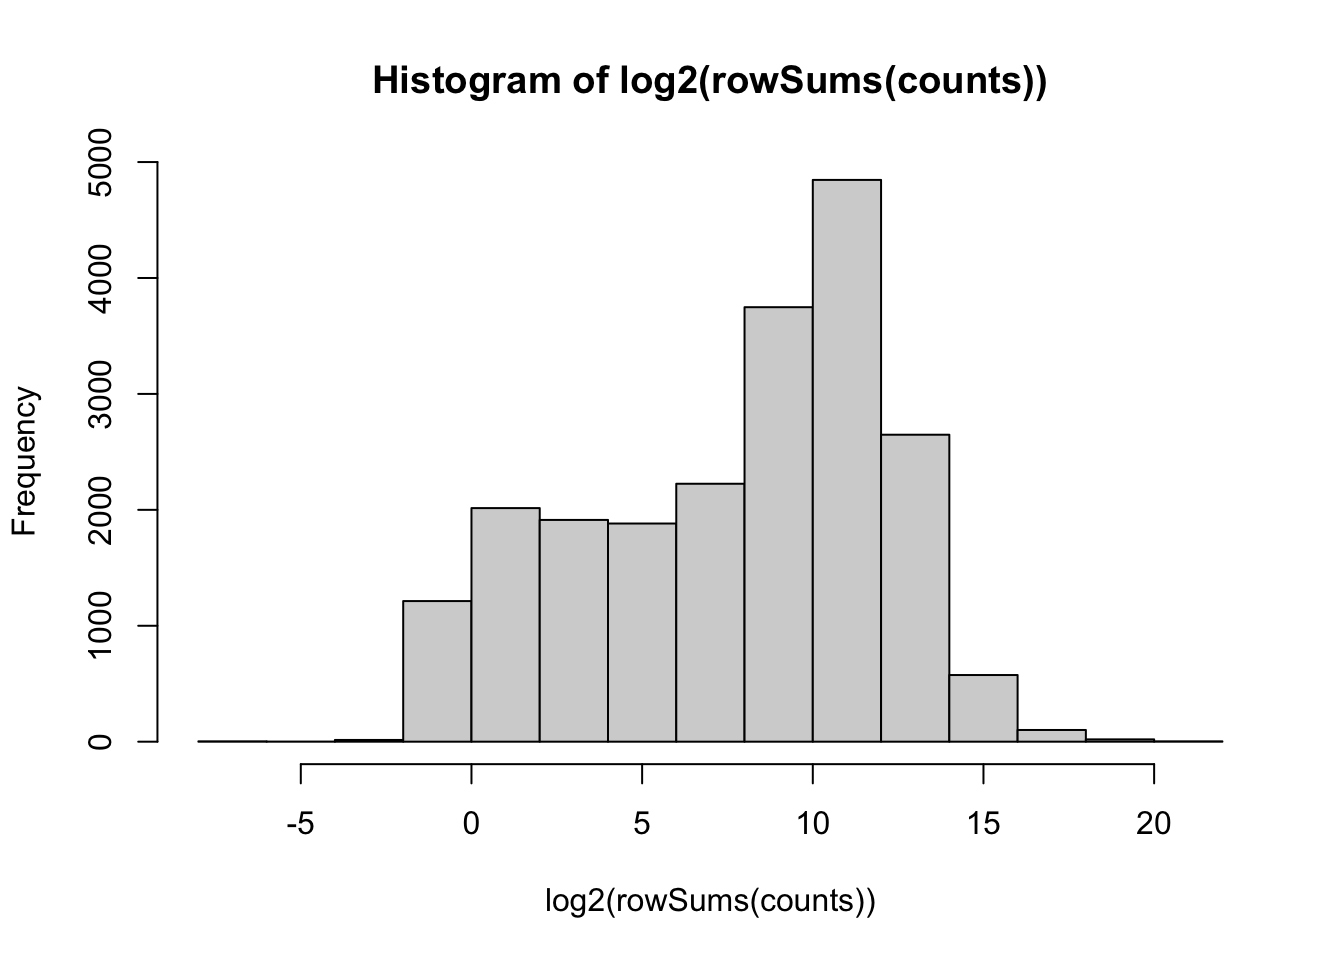
\includegraphics{Clean_files/figure-latex/unnamed-chunk-7-1.pdf}

\#\#\#3. Determine how many genes had zero counts and remove these genes
(rows) from the data set. What does your count distribution look like
before and after this?\#\#\#

\begin{Shaded}
\begin{Highlighting}[]
\NormalTok{MinVals }\OtherTok{\textless{}{-}} \FunctionTok{apply}\NormalTok{(counts, }\DecValTok{1}\NormalTok{, min)}
\FunctionTok{sum}\NormalTok{(MinVals }\SpecialCharTok{==} \DecValTok{0}\NormalTok{) }
\end{Highlighting}
\end{Shaded}

\begin{verbatim}
## [1] 24868
\end{verbatim}

\begin{Shaded}
\begin{Highlighting}[]
\NormalTok{Exp }\OtherTok{\textless{}{-}}\NormalTok{ counts[MinVals }\SpecialCharTok{\textgreater{}} \DecValTok{0}\NormalTok{, ]}
\end{Highlighting}
\end{Shaded}

\begin{Shaded}
\begin{Highlighting}[]
\NormalTok{ExpLog2 }\OtherTok{\textless{}{-}} \FunctionTok{log2}\NormalTok{(Exp)}
\FunctionTok{hist}\NormalTok{(}\FunctionTok{rowMeans}\NormalTok{(ExpLog2), }\AttributeTok{xlab =} \StringTok{"Counts (log2)"}\NormalTok{, }\AttributeTok{main =} \StringTok{"Expressed Genes"}\NormalTok{)}
\end{Highlighting}
\end{Shaded}

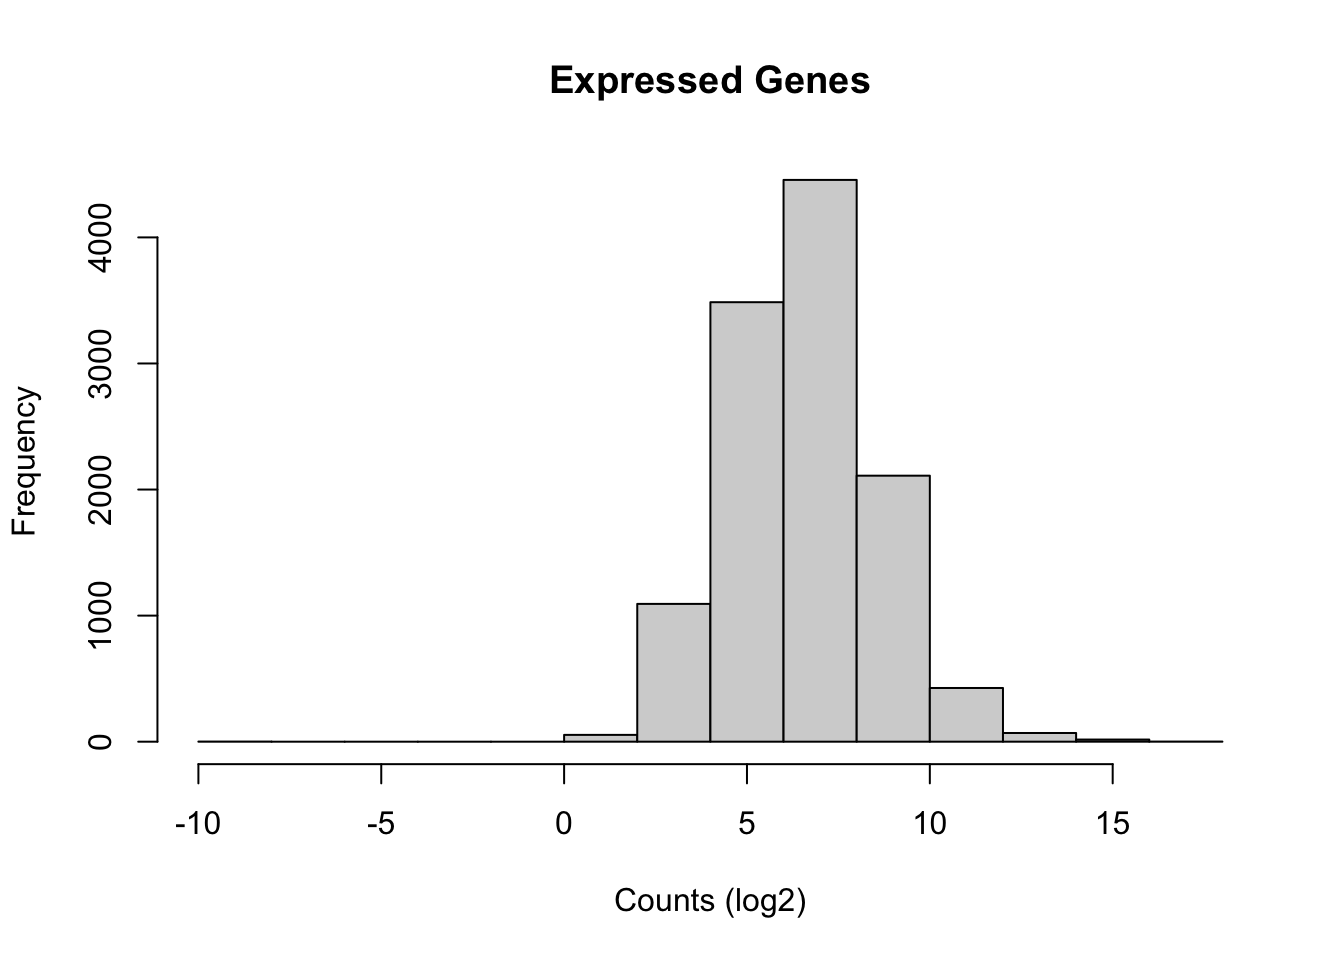
\includegraphics{Clean_files/figure-latex/unnamed-chunk-9-1.pdf}
\#\#\#4. Make a boxplot of log2 raw counts after removing all genes that
had zero counts.\#\#\#

Plot ``raw'' (our log2 transformed) sample counts

\begin{Shaded}
\begin{Highlighting}[]
\FunctionTok{boxplot}\NormalTok{(ExpLog2, }\AttributeTok{ylab =} \StringTok{"log2 counts"}\NormalTok{, }\AttributeTok{main =} \StringTok{"Raw RNA{-}Seq Counts"}\NormalTok{, }\AttributeTok{las =} \DecValTok{2}\NormalTok{)}
\end{Highlighting}
\end{Shaded}

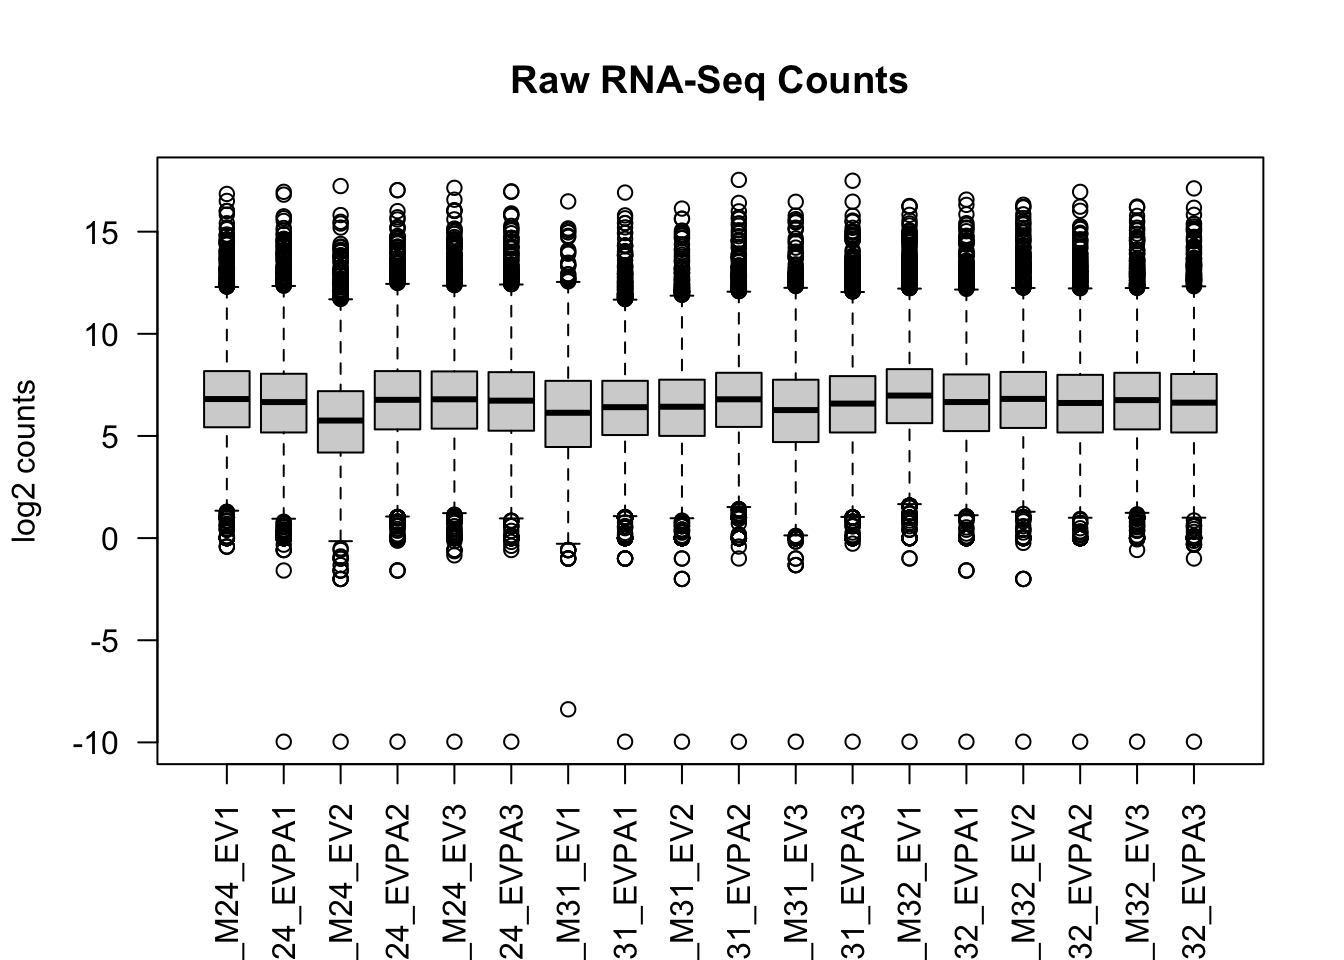
\includegraphics{Clean_files/figure-latex/unnamed-chunk-10-1.pdf}

\#\#\#5. Make a Cluster Dendrogram of the raw data.\#\#\#

\begin{Shaded}
\begin{Highlighting}[]
\NormalTok{RawDist }\OtherTok{\textless{}{-}} \FunctionTok{dist}\NormalTok{(}\FunctionTok{t}\NormalTok{(ExpLog2), }\AttributeTok{method =} \StringTok{"euclidean"}\NormalTok{)}
\FunctionTok{plot}\NormalTok{(}\FunctionTok{hclust}\NormalTok{(RawDist, }\AttributeTok{method =} \StringTok{"average"}\NormalTok{))}
\end{Highlighting}
\end{Shaded}

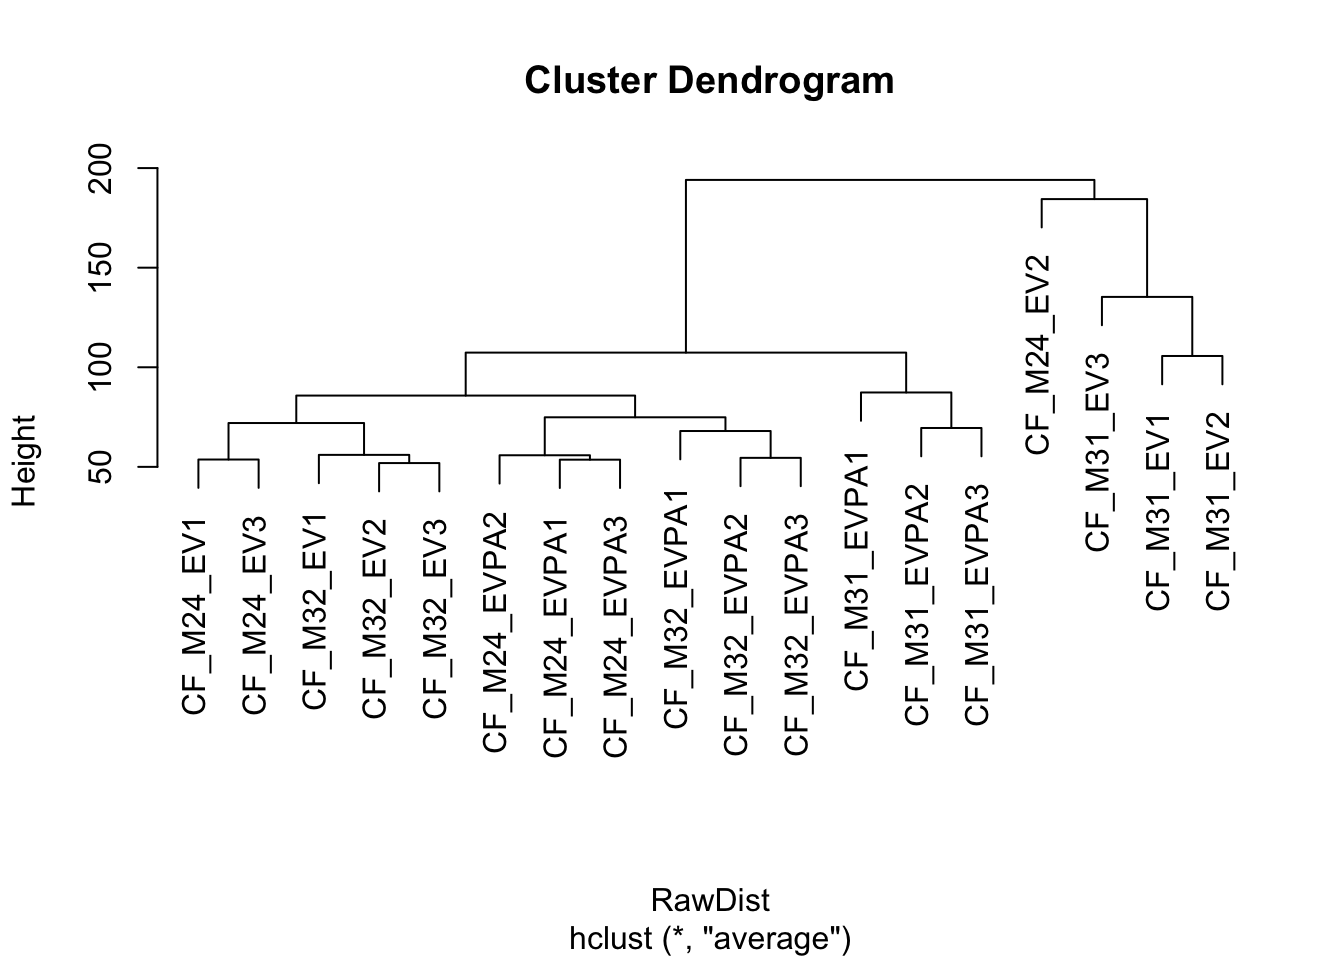
\includegraphics{Clean_files/figure-latex/unnamed-chunk-11-1.pdf}

Simple normalization

\begin{Shaded}
\begin{Highlighting}[]
\NormalTok{SampleMedians }\OtherTok{\textless{}{-}} \FunctionTok{apply}\NormalTok{(ExpLog2, }\DecValTok{2}\NormalTok{, median) }\CommentTok{\# Find the median value of each column {-} 2 means column}
\NormalTok{GrandMedian }\OtherTok{\textless{}{-}} \FunctionTok{mean}\NormalTok{(SampleMedians) }\CommentTok{\# Take the average of those}
\NormalTok{CorrectionFactors }\OtherTok{\textless{}{-}}\NormalTok{ GrandMedian }\SpecialCharTok{{-}}\NormalTok{ SampleMedians }\CommentTok{\# Calculate correction factor to apply to data}
\NormalTok{CorrectionFactors}
\end{Highlighting}
\end{Shaded}

\begin{verbatim}
##   CF_M24_EV1 CF_M24_EVPA1   CF_M24_EV2 CF_M24_EVPA2   CF_M24_EV3 CF_M24_EVPA3 
## -0.219473027 -0.070329588  0.832994393 -0.180937605 -0.206533972 -0.140038560 
##   CF_M31_EV1 CF_M31_EVPA1   CF_M31_EV2 CF_M31_EVPA2   CF_M31_EV3 CF_M31_EVPA3 
##  0.453085963  0.178490959  0.157864308 -0.206533972  0.321095354  0.002904366 
##   CF_M32_EV1 CF_M32_EVPA1   CF_M32_EV2 CF_M32_EVPA2   CF_M32_EV3 CF_M32_EVPA3 
## -0.389398029 -0.071942790 -0.225924944 -0.026827949 -0.167005607 -0.041489298
\end{verbatim}

These correction factors will align the medians of all of our samples
This changes our counts just enough to correct for variability between
samples/groups without loosing any actual effects of changes in gene
expression.

Loop through each column (sample) and fill in medians adjusted with
sample correction factor

\begin{Shaded}
\begin{Highlighting}[]
\NormalTok{ExpNorm }\OtherTok{\textless{}{-}}\NormalTok{ ExpLog2}

\ControlFlowTok{for}\NormalTok{(col }\ControlFlowTok{in} \FunctionTok{colnames}\NormalTok{(ExpNorm))\{}
\NormalTok{  ExpNorm[, col] }\OtherTok{\textless{}{-}}\NormalTok{ ExpLog2[, col] }\SpecialCharTok{+}\NormalTok{ CorrectionFactors[col]}
\NormalTok{\}}
\end{Highlighting}
\end{Shaded}

\begin{enumerate}
\def\labelenumi{\arabic{enumi}.}
\setcounter{enumi}{5}
\tightlist
\item
  Do a simple normalization of your data and visualize your normalized
  data with a boxplot of log2 raw counts and a cluster dendrogram. Did
  normalization change anything?
\end{enumerate}

\begin{Shaded}
\begin{Highlighting}[]
\FunctionTok{boxplot}\NormalTok{(ExpNorm, }\AttributeTok{ylab =} \StringTok{"log2 counts"}\NormalTok{, }\AttributeTok{main =} \StringTok{"Normalized Counts"}\NormalTok{, }\AttributeTok{las =} \DecValTok{2}\NormalTok{)}
\end{Highlighting}
\end{Shaded}

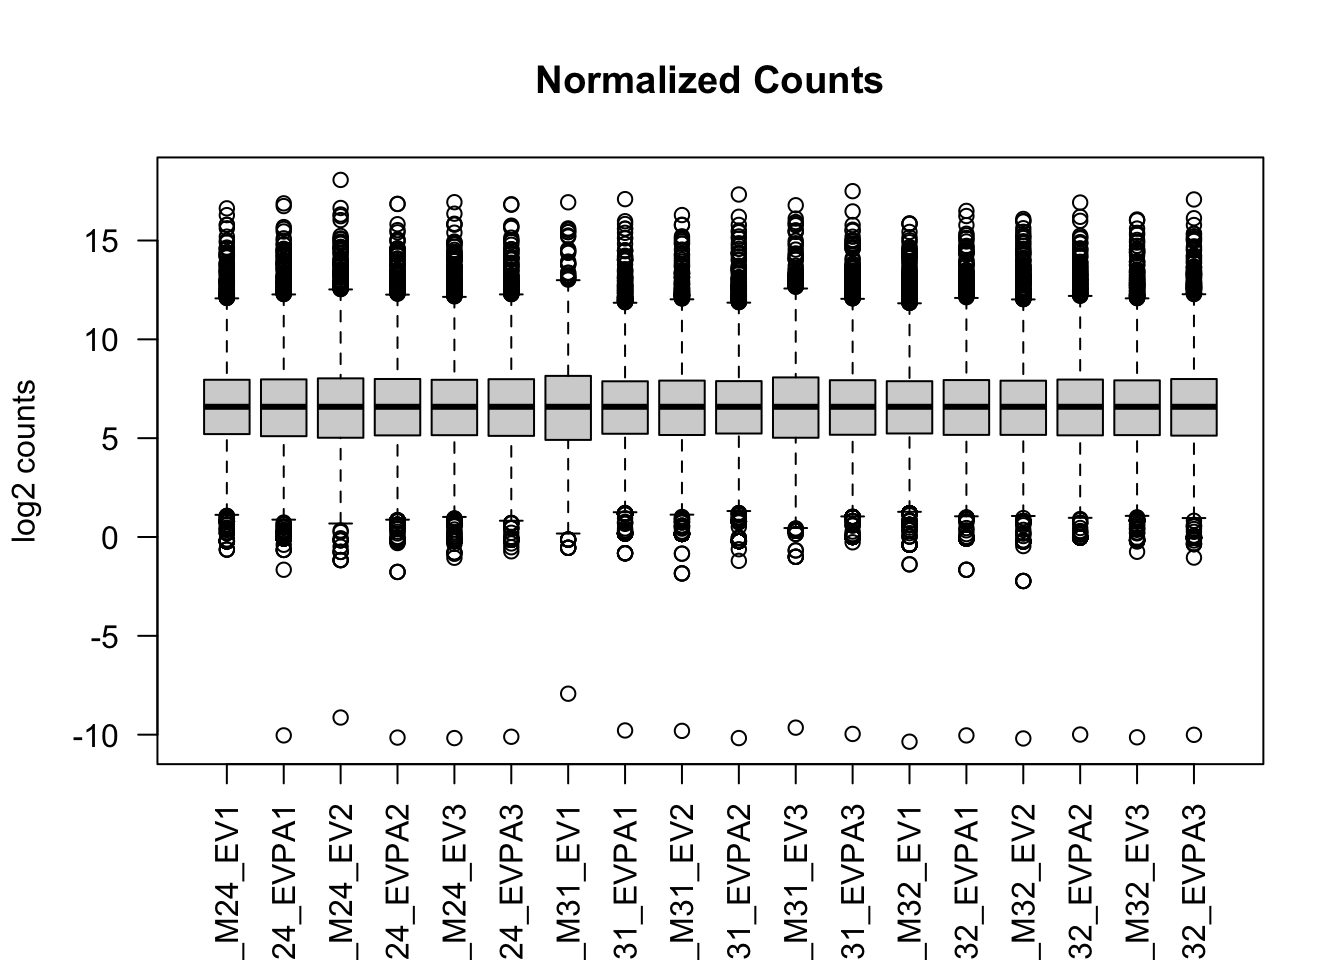
\includegraphics{Clean_files/figure-latex/unnamed-chunk-14-1.pdf}

Cluster dendrogram of normalized data

\begin{Shaded}
\begin{Highlighting}[]
\NormalTok{NormDist }\OtherTok{\textless{}{-}} \FunctionTok{dist}\NormalTok{(}\FunctionTok{t}\NormalTok{(ExpNorm), }\AttributeTok{method =} \StringTok{"euclidean"}\NormalTok{)}
\FunctionTok{plot}\NormalTok{(}\FunctionTok{hclust}\NormalTok{(NormDist, }\AttributeTok{method =} \StringTok{"average"}\NormalTok{))}
\end{Highlighting}
\end{Shaded}

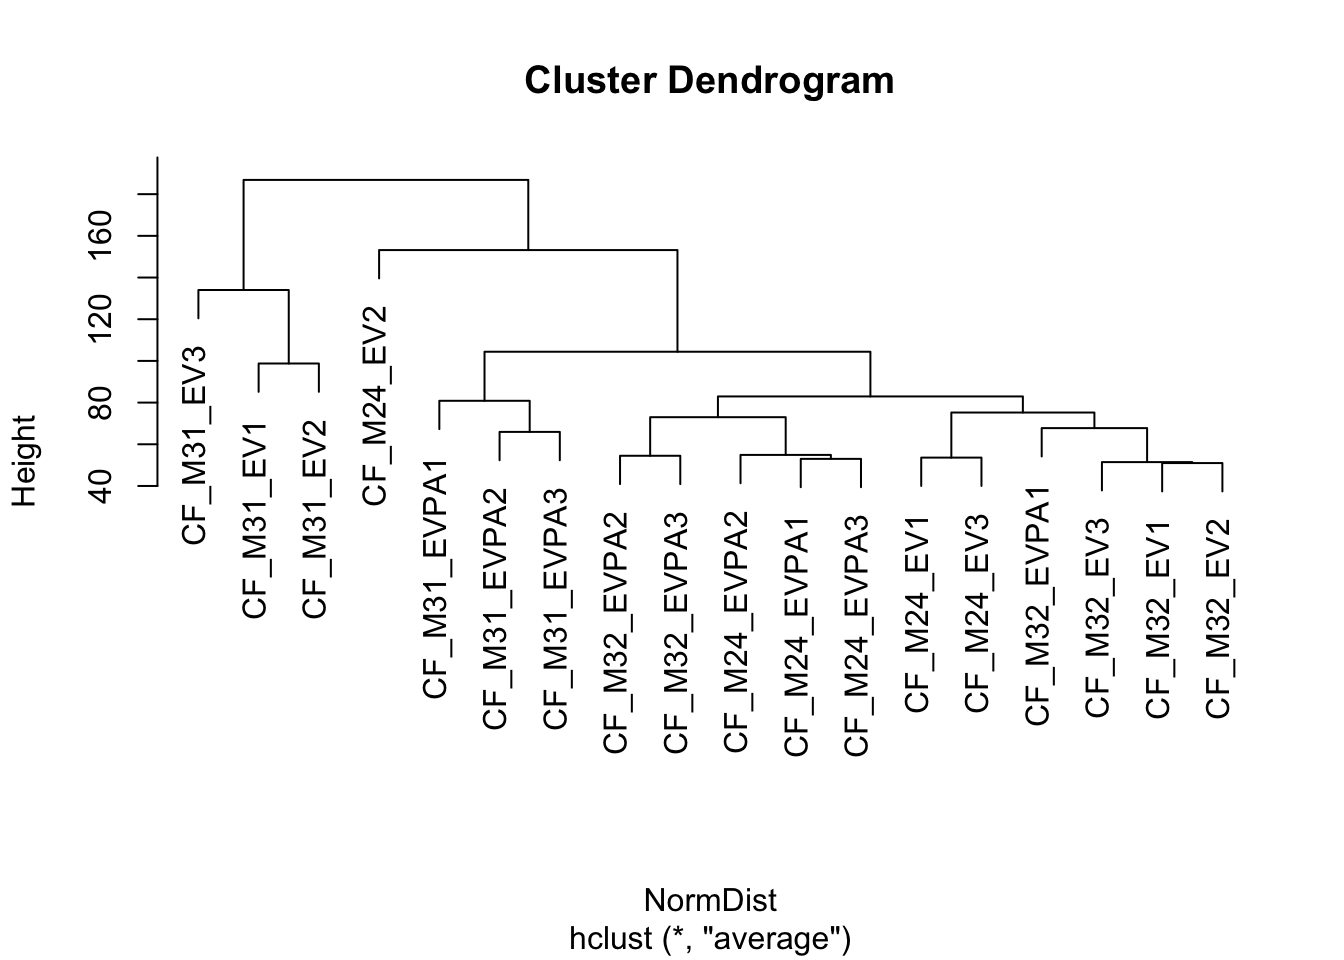
\includegraphics{Clean_files/figure-latex/unnamed-chunk-15-1.pdf} \#\#\#
7.Make a PCA plot and use color to highlight groups. \#\#\#

\begin{Shaded}
\begin{Highlighting}[]
\NormalTok{PCA }\OtherTok{\textless{}{-}} \FunctionTok{prcomp}\NormalTok{(}\FunctionTok{t}\NormalTok{(NormDist))}
\FunctionTok{plot}\NormalTok{(PCA}\SpecialCharTok{$}\NormalTok{x[ , }\DecValTok{1}\NormalTok{], PCA}\SpecialCharTok{$}\NormalTok{x[ , }\DecValTok{2}\NormalTok{], }\AttributeTok{pch =} \DecValTok{16}\NormalTok{)}
\end{Highlighting}
\end{Shaded}

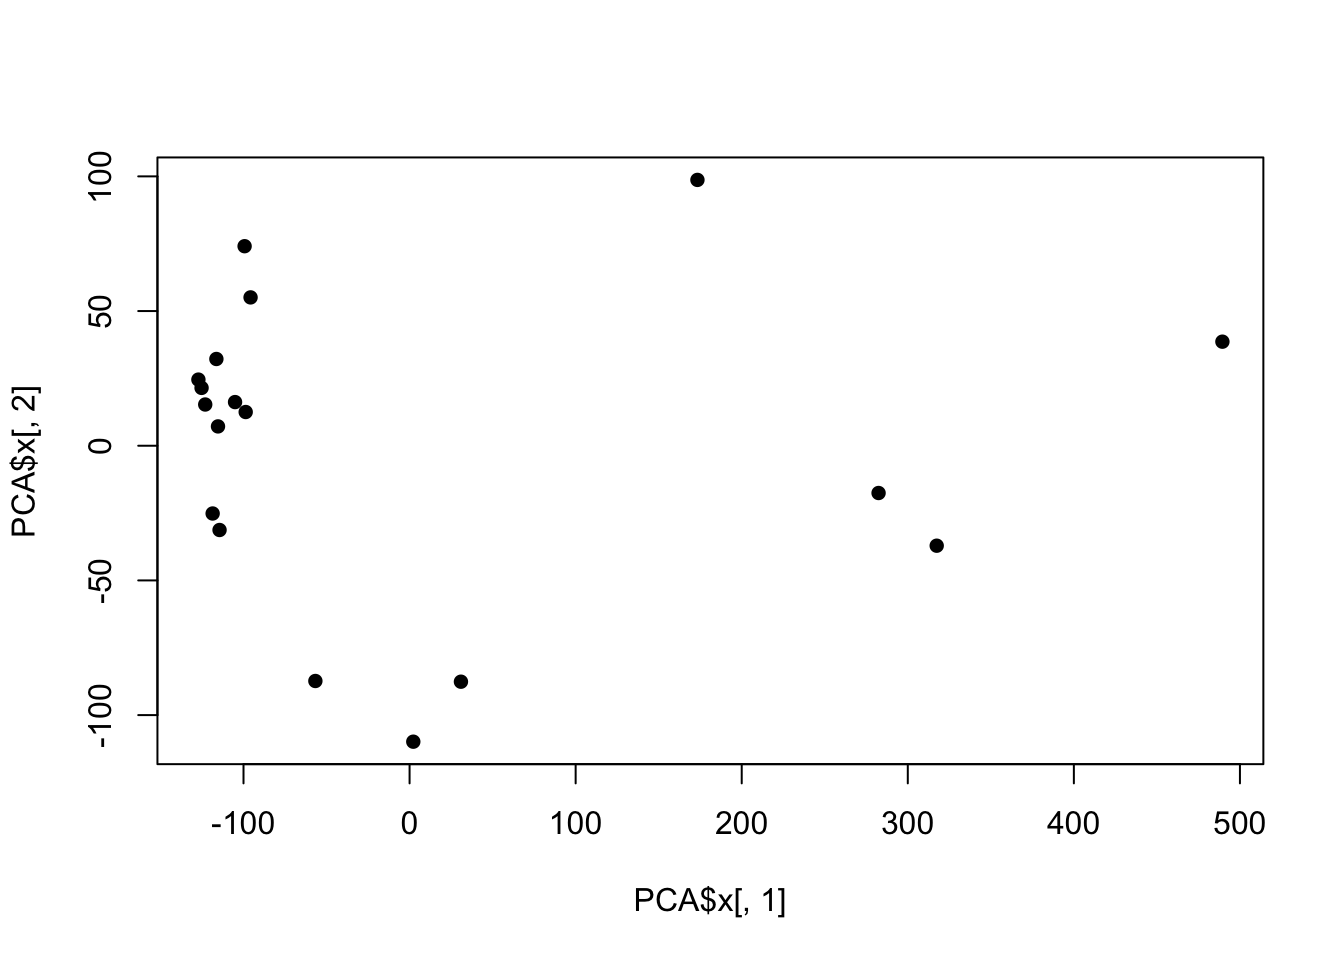
\includegraphics{Clean_files/figure-latex/unnamed-chunk-16-1.pdf}

By donor

\begin{Shaded}
\begin{Highlighting}[]
\FunctionTok{plot}\NormalTok{(PCA}\SpecialCharTok{$}\NormalTok{x[ , }\DecValTok{1}\NormalTok{], PCA}\SpecialCharTok{$}\NormalTok{x[ , }\DecValTok{2}\NormalTok{], }\AttributeTok{pch =} \DecValTok{16}\NormalTok{, }\AttributeTok{col =}\NormalTok{ donors, }
     \AttributeTok{main =} \StringTok{"Colored by Donor"}\NormalTok{)}
\FunctionTok{legend}\NormalTok{(}\StringTok{"bottomright"}\NormalTok{, }\AttributeTok{legend =} \FunctionTok{unique}\NormalTok{(donors), }\AttributeTok{pch =} \DecValTok{16}\NormalTok{, }\AttributeTok{col =} \FunctionTok{unique}\NormalTok{(donors))}
\end{Highlighting}
\end{Shaded}

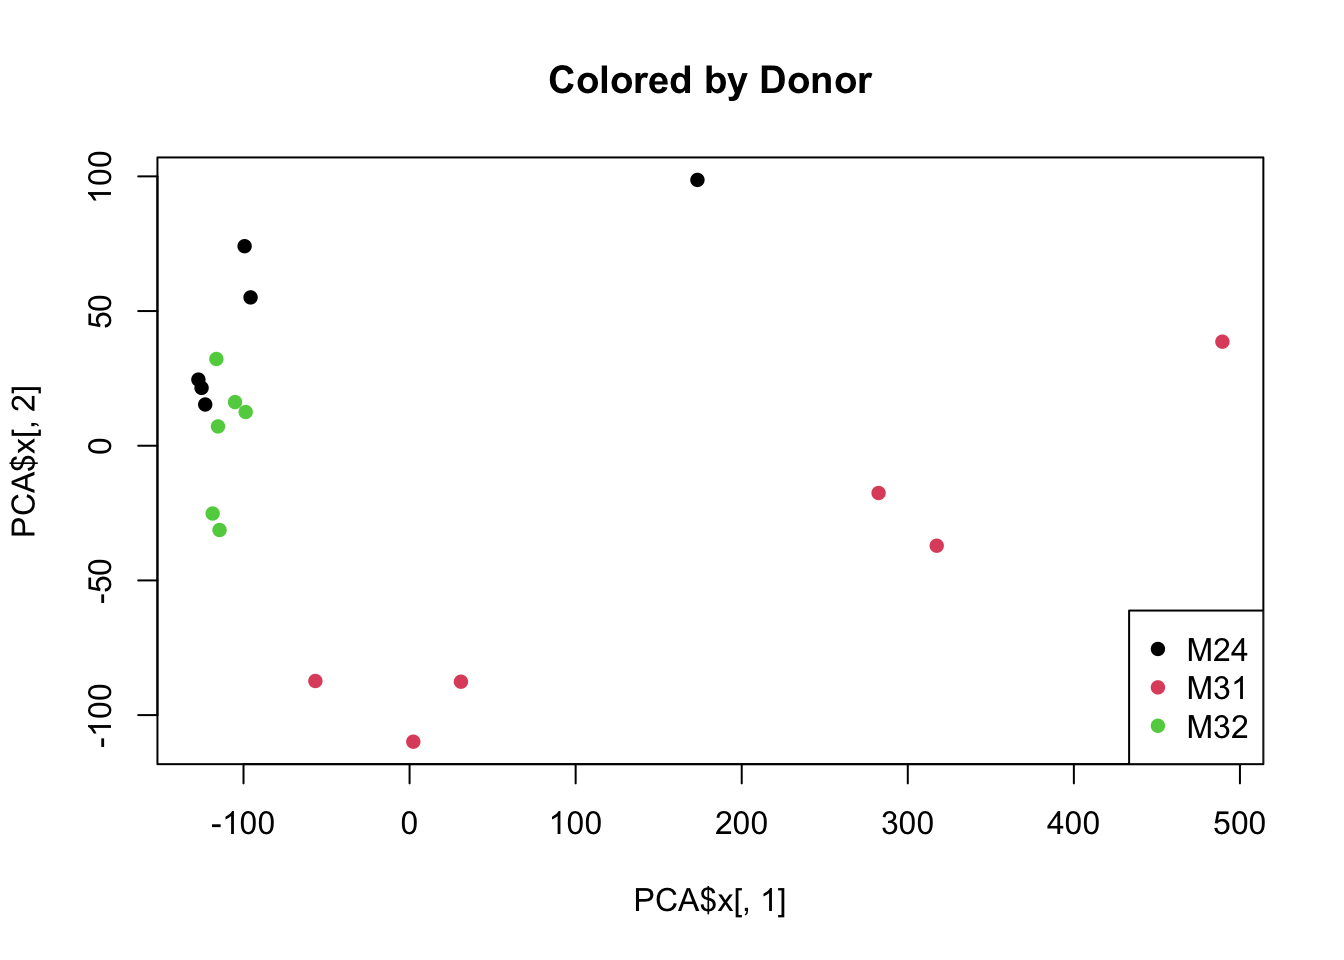
\includegraphics{Clean_files/figure-latex/unnamed-chunk-17-1.pdf} By
treatment

\begin{Shaded}
\begin{Highlighting}[]
\FunctionTok{plot}\NormalTok{(PCA}\SpecialCharTok{$}\NormalTok{x[ , }\DecValTok{1}\NormalTok{], PCA}\SpecialCharTok{$}\NormalTok{x[ , }\DecValTok{2}\NormalTok{], }\AttributeTok{pch =} \DecValTok{16}\NormalTok{, }\AttributeTok{col =}\NormalTok{ treatment, }
     \AttributeTok{main =} \StringTok{"Colored by Treatment"}\NormalTok{)}
\FunctionTok{legend}\NormalTok{(}\StringTok{"bottomright"}\NormalTok{, }\AttributeTok{legend =} \FunctionTok{unique}\NormalTok{(treatment), }\AttributeTok{pch =} \DecValTok{16}\NormalTok{, }\AttributeTok{col =} \FunctionTok{unique}\NormalTok{(treatment))}
\end{Highlighting}
\end{Shaded}

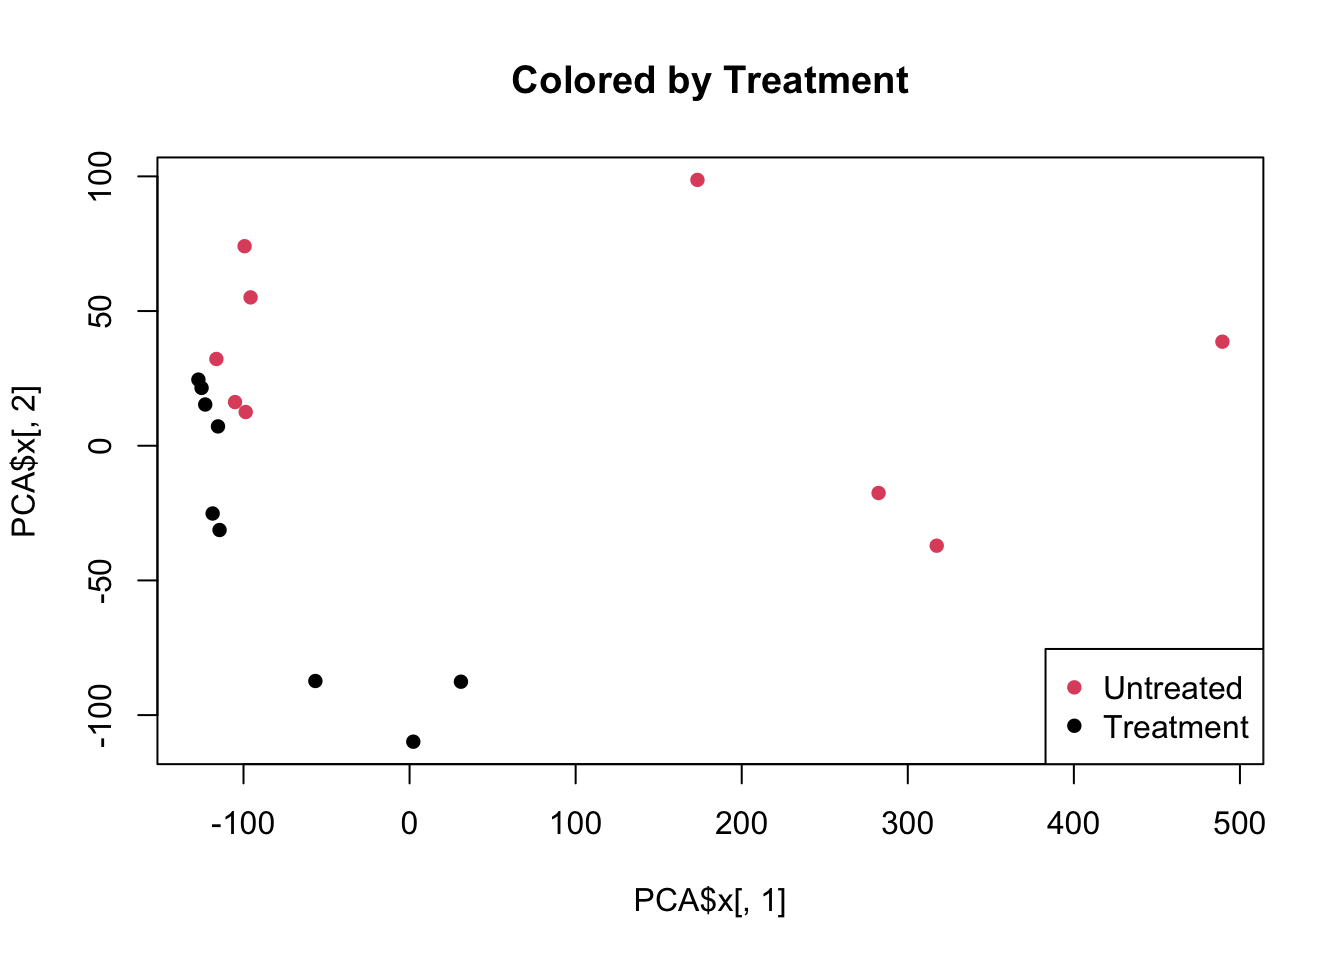
\includegraphics{Clean_files/figure-latex/unnamed-chunk-18-1.pdf}

\end{document}
